\begin{figure}[p]
\centering
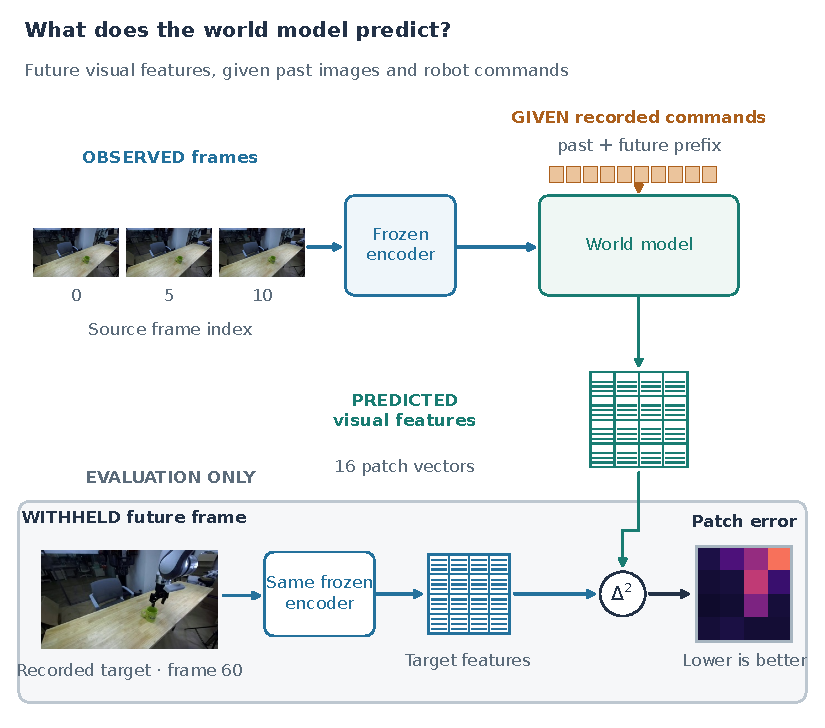
\includegraphics[width=\linewidth]{generated/real_video/spatial_task.pdf}
\caption{\textbf{The recorded-video prediction task.} The model receives three observed images and recorded robot commands, then forecasts visual-feature vectors for a future time. The withheld future RGB frame is used only for evaluation: the same frozen DINO encoder supplies its target features, which are compared with the forecast. The model outputs features, not a generated RGB frame or a chosen robot action. The 16 vector glyphs denote feature vectors schematically; the final heatmap is the actual three-seed $h=10$ per-patch standardized feature error for the prespecified median episode's first window (mean MSE 0.1727; one shared scale 0--0.787 across the companion gallery). Bright patches have larger feature error; this is not a pixel-reconstruction error map. The example's episode-average gain is +5.358\%, but this fixed displayed window has a -0.305\% gain against the autoregressive baseline. Recorded images are unchanged DROID observations (CC BY 4.0); the target frame never enters the forecasting model.}
\label{fig:spatial-task}
\end{figure}
